\chapter{Resultados y discusión}

Uno de los objetivos principales de esta tesis fue desarrollar un programa de cómputo científico para explorar la posible aplicación del análisis multifractal en estructuras proteicas, por lo tanto, el programa podría ser una herramienta útil para caracterizar las distintas etapas del plegamiento proteico, describiéndolas en términos de la dinámica de formación de agregados estructurales, lo que permitiría una comprensión más profunda de estos procesos. Para mejorar la compresión de este trabajo, se ha dividido la descripción del programa \textit{\textbf{molmassfractraldim}} en dos secciones; el algoritmo y su uso para la obtención de resultados. 
 
 
\section{Algoritmo (diseño del programa)}

El propósito principal del programa \textbf{\textit{molmassfractaldim}} es determinar la dimesi\'{o}n fractal de masa mediante la caracterizaci\'{o}n de la geometría interna de un sistema proteico. Esto se logra construyendo una tabla de \(r_i\), \( \bar{N}(r_i)\), \( \bar{M}(r_i)\) y  \( {Rg}(r_i)\) donde;

\begin{itemize}
	\item \(r_i\) es el radio de medida centrado en posiciones aleatorias de una prote\'{i}na con valores m\'{i}nimos y m\'{a}ximos definidos como \(mr_{min}\) y \(mr_{max}\).
	\item \(\bar{N}(r_i)\) es el número promedio de partículas contenidas dentro de un radio \(r_i\). 
	\item  \(\bar{M}(r_i)\) es el n\'{u}mero de masa promedio de las part\'{i}culas contenidas en el radio \(r_i\).
	\item  \({Rg}(r_i)\) es el radio de giro promedio de las part\'{i}culas contenidas en el radio \(r_i\).
\end{itemize}

Posteriormente, los valores de \( \bar{N}(r_i) \), \( \bar{M}(r_i)\) y \({Rg}(r_i)\) pueden analizarse mediante regresiones lineales para determinar la dimensi\'{o}n fractal de masa. El procedimiento general del programa \textbf{\textit{molmassfractaldim}} se describe en el diagrama de flujo de la figura \ref{dfMolFractalDim}, cuyos pasos se explican a detalle en las siguientes subsecciones.
 
 
 \begin{figure}[h!]
 	\begin{center}
 		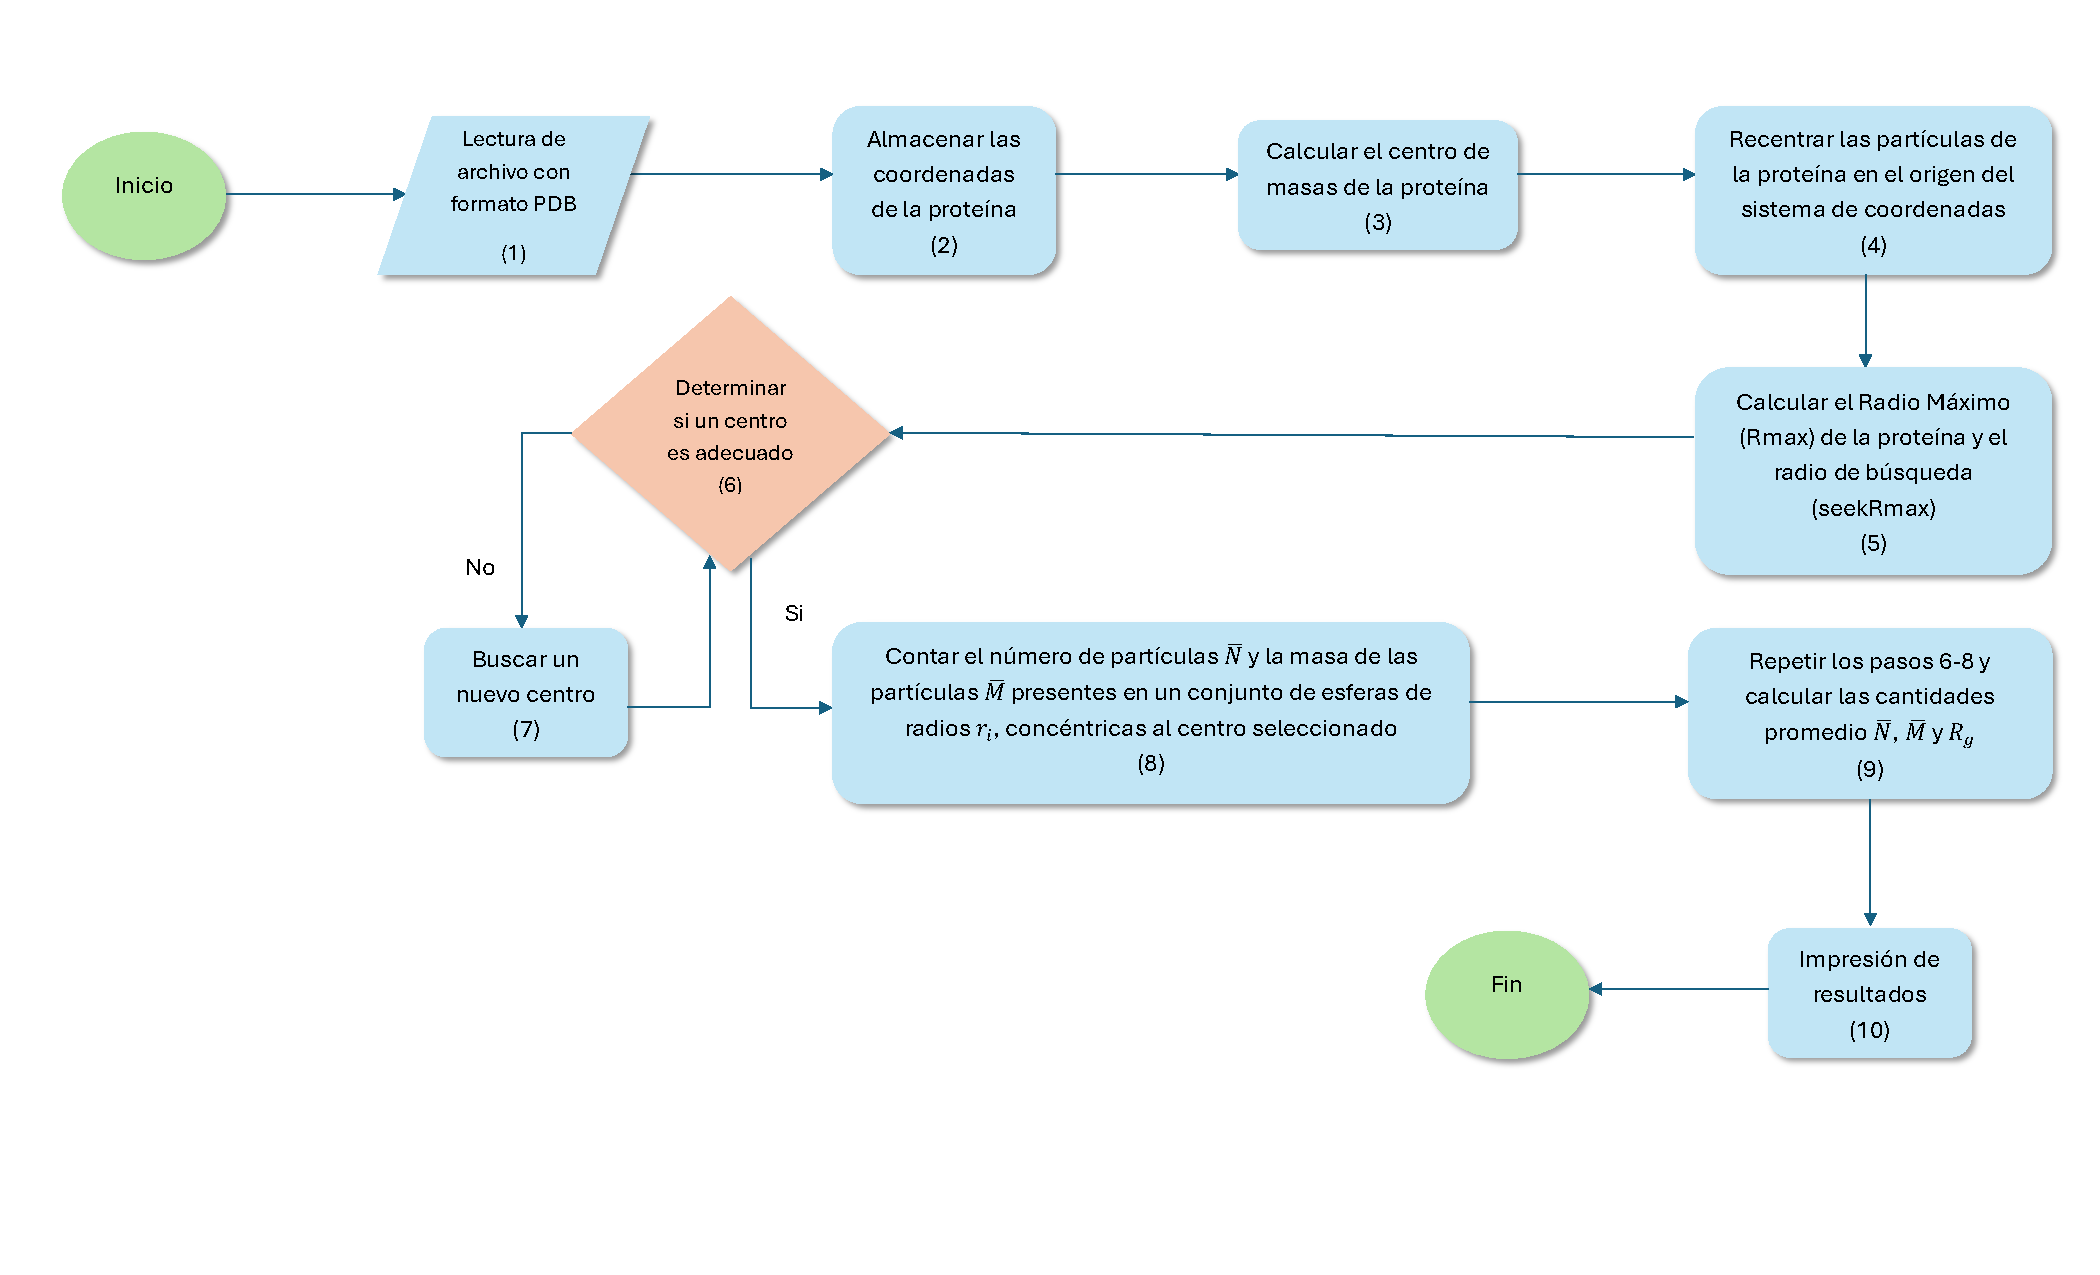
\includegraphics[width=\textwidth]{graphs/dfMolFractalDim}
 		\caption{Diagrama de flujo general del programa \textit{molmassfractaldim}.}
 		\label{dfMolFractalDim}
 	\end{center}
 \end{figure}
 
 
 \subsection {Pasos 1, 2, 3 y 4 del diagrama de flujo general}
 
	\begin{itemize}
		\item \textbf{Paso 1}:  El programa \textbf{\textit{molmassfractaldim}} inicia con el
		uso de una clase llamada \textit{InputMoleculePDB} que se encargar de realizar 
		la lectura de un archivo en formato \textit{PDB}  para filtrar las líneas que 
		comienzan con \texttt{ATOM} o \texttt{HETATM} y así, extraer datos 
		fundamentales para el programa como:  
		
		\begin{itemize}
			\item Número atómico (\texttt{atomicNumber}) de cada átomo.
			\item Coordenadas cartesianas \((x_i, y_i, z_i)\) en \AA ngstr\"oms.
			\item Masa atómica (\texttt{atomicMass}) de cada átomo.
			\item Número total de átomos (\texttt{natoms}) en la proteína.
		\end{itemize}
		Estos datos son almacenados en vectores internos (\texttt{atomNumbers[]}, \texttt{coords[]}, \texttt{masses[]}) 
		que serán utilizados por otros módulos.
	
		\item \textbf{Paso 2}: 	A partir de los datos leídos, se crea un objeto de una clase llamada \textit{Molecule},
		la cual internamente almacena la información estructural en tres vectores principales:
		
		\begin{itemize}
			\item \texttt{X[]}, \texttt{Y[]}, \texttt{Z[]} para coordenadas atómicas.
			\item \texttt{atomicNumber[]} para los números atómicos.
			\item \texttt{mass[]} para las masas atómicas.
		\end{itemize}
		

		En este paso, la función \texttt{setCoordinates()} copia los valores de \textit{InputMoleculePDB}
		 a los vectores internos de \textit{Molecule}.
		
		
		\item \textbf{Paso 3}: Nuevamente se usa la clase 
		\textit{Molecule} para el cálculo de propiedades moleculares como:
		
		\begin{itemize}
			\item Determinar la fórmula empírica de la molécula, contado la cantidad de átomos por número atómico.
			\item Devolver valores como la cantidad de átomos de un tipo específico 
			dado por el número átomico.
			\item Calcular los extremos mínimos y máximos de todos los átomos para definir 
			el radio máximo desde el origen de la esfera que envuelve a la proteína.
			\item Calcula el centro de masa considerando las masas atómicas.
			\item Calcula el centroide (promedio aritmético de las coordenadas de todos los
			átomos, sin considerar su masa).
		\end{itemize}
		
		Por último en este paso, la clase \textit{Molecule} también se encarga de trasladar 
		la proteína de modo que su centroide coincida con el origen de las coordenas \((0, 0, 0)\).  
		
		
		\item \textbf{Paso 4}: En este paso la clase \textit{Molecule} se encarga de identificar 
		enlaces covalentes entre átomos según la distancia que exista entre ellos y sus radios 
		de Van Der Waals (ecuación \ref{dij}) para devolver una lista con los índices de vecinos cercanos a un átomo dado.
		A continuación se detalla el paso 4:
				
		\begin{enumerate}
			\item Calcula la distancia \(d_{ij}\) entre el átomo \(i\) y el átomo \(j\):

			\begin{equation}
							d_{ij} = \sqrt{ (x_i - x_j)^2 + (y_i - y_j)^2 + (z_i - z_j)^2 }
							\label{dij}
			\end{equation}
			
			\item Compara \(d_{ij}\) con la suma de los radios de Van der Waals de ambos átomos.
			\item Si \(d_{ij} \leq r^{vdW}_i + r^{vdW}_j + \epsilon\), se agrega \(j\) a la lista de vecinos de \(i\).
		\end{enumerate}
		
	\end{itemize}


	\subsection{Paso 5 del diagrama de flujo general}
	
	En este paso una nueva clase llamada \textit{massfractaldim} determina el radio máximo de la 
	proteína (\(R_{max}\)), calculado como la distancia máxima desde el origen \(x, y, z\) hasta 
	cualquier átomo de la molécula. Matemáticamente esto se escribe como:
	
	\begin{equation}
		R_{max} = max_{i} \sqrt{x^{2}_{i} + y^{2}_{i} + z^{2}_{i}}
	\end{equation}
 	
 	Donde \(x_{i}, y_{i}, z_{i}\) representan las coordenadas cartesianas de un conjunto de átomos 
 	en tres dimensiones. Ejemplo: Supóngase la existencia de 5 átomos con las siguientes 
 	coordenadas en 3D:
 	
 	\begin{table}[h!]
 		\centering
 		\begin{tabular}{ccccc}
 			\textbf{Átomo \(i\)} & \textbf{\(x_i\)} & \textbf{\(y_i\)} & \textbf{\(z_i\)} & \(R_{max}= \sqrt{x_i^2 + y_i^2 + z_i^2}\) \\
 			\hline
 			1 & 1.0 & 0.5 & 2.0 & \(\sqrt{1^2 + 0.5^2 + 2^2} = 2.29\) \\
 			2 & -0.5 & 1.0 & -1.5 & \(\sqrt{(-0.5)^2 + 1^2 + (-1.5)^2} = 1.87\) \\
 			3 & 0.0 & -2.0 & 1.0 & \(\sqrt{0^2 + (-2)^2 + 1^2} = 2.23\) \\
 			4 & 2.0 & 1.5 & 0.5 & \(\sqrt{2^2 + 1.5^2 + 0.5^2} = 2.54\) \\
 			5 & -1.0 & -1.0 & -2.5 & \(\sqrt{(-1)^2 + (-1)^2 + (-2.5)^2} = 2.87\) \\
 		\end{tabular}
 		\caption{Cálculo de la distancia radial \(r_i\) para 5 átomos.}
 	\end{table}
 	
 	Por lo tanto, el \textbf{radio máximo} 
 	es: \textbf{\(R_{max}\) = max\(\{2.29, 1.87, 2.23, 2.54, 2.87\}\) = 2.87}
 	
 	Hecho lo anterior, en esta misma clase se define un radio dentro del cual se buscan puntos
 	 de medición adecuados para analizar la distribución de masa. A este radio se le conoce
 	  como $seekRmax$ que a través de un condicional de tipo \textit{if} se asegura que el valor 
 	  de \textit{seekRmax} tenga un valor por defecto de $75\%$ tamaño del clúster (proteína), 
 	  salvo que el usuario especifique otro valor.
 	
 	\begin{equation}
 		 	seekRmax = 0.75 \times R_{max} 
 	\end{equation}
 	
 	Otros usos que tiene \textit{seekRmax} son:
 	
 	\begin{itemize}
 		\item Se asegura de que los puntos de medición no estén demasiado cerca de los límites del clúster.
 		\item Evita que los círculos de medición se salgan del clúster.
 		\item Evita tomar semillas demasiado cerca de los bordes del clúster.
 		\item Ayuda a definir los radios mínimo y máximo de medición: $mr_{min}$ y $mr_{max}$.
 	\end{itemize}
 
 	Posteriormente, se define el número de radios de medición como \(nr = 50\) y el incremento radial \(dr\) 
 	para  generar un vector \(r_i\) con valores \(mr_{min}= 0.5\) hasta \(mr_{max} = 20\), en incrementos de \(dr\):
 
 	\begin{equation}
 		 	dr = \frac{mr_{max} - mr_{min}}{nr - 1}
 	\end{equation}
	
	 Después, se define el n\'{u}mero de medidas por centro como \(nMeas = 30\) y el n\'{u}mero total 
	 de c\'{i}rculos a considerar.
	 
	 
	 \subsection{Paso 6 y 7 del diagrama de flujo general}
	 
	 
	 En este paso se crea un criterio para calcular si un centro local es adecuado y sirve para determinar si una esfera de cierto radio, centrada en alg\'{u}n \'{a}tomo de la prote\'{i}na, intersecta de manera importante un hueco en la estructura proteica. Además, permite refinar la medici\'{o}n de la relaci\'{o}n \( \bar{N}(r_i) \), \( \bar{M}(r_i)\) y \({Rg}(r_i)\), que a su vez es la relaci\'{o}n que se utiliza para medir la dimensión fractal en estructuras proteicas. Este criterio calcula dos valores clave que son el volumen de cada esfera de radio \(r_i\) y la densidad de partículas promedio presente en cada esfera de radio \(r_i\). El volumen de cada esfera se calcula usando el radio \(r_i\) de las esferas definidas anteriormente y a partir de la ecuaci\'{o}n \ref{volumen}.\\
	 
	 \begin{equation}
	 	V(r_i) = \frac{4}{3} \pi r_{i}^{3}
	 	\label{volumen}
	 \end{equation}
	 
	 La densidad de part\'{i}culas promedio se calcula a partir de la ecuaci\'{o}n \ref{eq:densidad}. \\
	 Donde \(\rho_{P}\) es la densidad de part\'{i}culas promedio presentes en una esfera de radio \(r_i\).\\
	 \(\bar N(r_{i})\) es la cantidad promedio de part\'{i}culas presentes en una esfera de radio \(r_i\).
	 \(V_{i}\) es el volumen de una esfera de radio \(r_{i}\).
	 
	 \begin{equation}
	 	\rho_P = \frac{\bar N(r_{i})}{V_{i}}
	 	\label{eq:densidad}
	 \end{equation}
	 
	 El criterio  servir\'{a} para determinar si una esfera de cierto radio, centrada en alg\'{u}n \'{a}tomo de la prote\'{i}na, intersecta de manera importante un hueco en la estructura proteica. Esto nos ser\'{a} \'{u}til para refinar la medici\'{o}n de la relaci\'{o}n $\bar N(r_i)$, que a su vez es la relaci\'{o}n que utilizaremos para medir dimensiones fractales y as\'{i}, determinar si existe o no multifractalidad en la estructura de las prote\'{i}na.
	 

	\subsection{Paso 8 del diagrama de flujo general}
 
	Para cada radio \(r_i\), acumula:
	
	\begin{equation}
			\bar{N}(r_i) = \frac{1}{N_c} \sum_{c=1}^{N_c} N_c(r_i), \quad
		\bar{M}(r_i) = \frac{1}{N_c} \sum_{c=1}^{N_c} M_c(r_i)
	\end{equation}

	Donde \(N_c(r_i)\) y \(M_c(r_i)\) son el conteo de partículas y la suma de masas 
	dentro de \(r_i\) desde el centro \(c\), y \(N_c\) es el número de centros de medida.

	 Generaci\'{o}n de puntos de medida\\
	Se eligen de manera aleatoria part\'{i}culas del sistema como centros de las circunferencias de medida. Para cada centro, se identifican las part\'{i}culas contenidas dentro del radio m\'{a}ximo (\(R_{max}\)).
	
	Acumulaci\'{o}n de datos\\
	Para cada radio \( r_i \), se cuenta cu\'{a}ntas part\'{i}culas est\'{a}n contenidas dentro de ese radio respecto al centro actual. Esta cuenta se repite para m\'{u}ltiples centros y se promedia para obtener \(\bar{N}(r_i)\).


 	
 	\subsection{Paso 9 del diagrama de flujo general}
 		

 	Para cada radio \( r_i \), se cuenta cu\'{a}ntas part\'{i}culas est\'{a}n contenidas dentro de ese radio respecto al centro actual. Esta cuenta se repite para m\'{u}ltiples centros y se promedia para obtener \( \bar{N}(r_i) \)	y se prepara un vector de resultados .
 
 
 	\clearpage
 
	\begin{comment}
		\begin{enumerate}
			\item Inicializaci\'{o}n\\
			Se carga un objeto llamado Molecule que contiene la informaci\'{o}n estructural del sistema (coordenadas y masas de los elementos presentes en la prote\'{i}na).
			
			\item Configuraci\'{o}n de par\'{a}metros\\
			Se calcula el centro de masas del cl\'{u}ster.\\
			Se recentran las part\'{i}culas de la prote\'{i}na en el origen del sistema de coordenadas.\\
			Se define el radio m\'{a}ximo del cluster \(R_{max}\) (la mayor distancia entre un \'{a}tomo y el origen).\\
			Se define el radio m\'{a}ximo de b\'{u}squeda de semillas como \(seekR_{max}\) para evitar que los c\'{i}rculos de medici\'{o}n se salgan del cl\'{u}ster.\\
			Se definen los radios m\'{i}nimo y m\'{a}ximo de medida como \(mr_{min}\) y \(mr_{max}\).\\
			Se calcula el n\'{u}mero de divisiones como \(nr\) y el incremento radial \(dr\).\\
			Se define el n\'{u}mero de medidas por centro como nMeas y el n\'{u}mero total de c\'{i}rculos a considerar.
			
			\item Generaci\'{o}n de puntos de medida\\
			Se eligen de manera aleatoria part\'{i}culas del sistema como centros de las circunferencias de medida. Para cada centro, se identifican las part\'{i}culas contenidas dentro del radio m\'{a}ximo (\(R_{max}\)).
			
			\item Acumulaci\'{o}n de datos\\
			Para cada radio \( r_i \), se cuenta cu\'{a}ntas part\'{i}culas est\'{a}n contenidas dentro de ese radio respecto al centro actual. Esta cuenta se repite para m\'{u}ltiples centros y se promedia para obtener \( \bar{N}(r_i) \).
			
		\end{enumerate}
	\end{comment}
 
 

	\begin{comment}
		
		\subsection{Pasos 1, 2, 3 y 4 del diagrama de flujo general}
	
			
		
			
			\item \textbf{Paso 3}:  
			La clase \textit{Molecule} ejecuta una serie de métodos para calcular propiedades moleculares:
			\begin{itemize}
				\item \texttt{calculateFormula()} — Recorre \texttt{atomicNumber[]} y construye un mapa clave-valor \{número atómico : cantidad\}.
				\item \texttt{countAtoms(atomicNum)} — Retorna el conteo de átomos con número atómico igual a \texttt{atomicNum}.
				\item \texttt{calculateBoundingBox()} — Obtiene mínimos y máximos de $x, y, z$ para determinar el tamaño del clúster.
				\item \texttt{centerOfMass()} — Calcula:
				\[
				CM_x = \frac{\sum_{i=1}^{N} m_i x_i}{\sum_{i=1}^{N} m_i}, \quad
				CM_y = \frac{\sum_{i=1}^{N} m_i y_i}{\sum_{i=1}^{N} m_i}, \quad
				CM_z = \frac{\sum_{i=1}^{N} m_i z_i}{\sum_{i=1}^{N} m_i}
				\]
				\item \texttt{centroid()} — Calcula el promedio aritmético de coordenadas sin ponderar por masa.
				\item \texttt{translateToOrigin()} — Resta las coordenadas del centroide a todas las posiciones $(x_i, y_i, z_i)$, trasladando la proteína al origen $(0,0,0)$.
			\end{itemize}
			
			\item \textbf{Paso 4}:  
			La clase \textit{Molecule} ejecuta \texttt{findNeighbors(atomIndex, cutoff)} para detectar enlaces covalentes:
			\begin{enumerate}
				\item Calcula la distancia $d_{ij}$ entre el átomo $i$ y el átomo $j$:
				\[
				d_{ij} = \sqrt{ (x_i - x_j)^2 + (y_i - y_j)^2 + (z_i - z_j)^2 }
				\]
				\item Compara $d_{ij}$ con la suma de los radios de Van der Waals de ambos átomos.
				\item Si $d_{ij} \leq r^{vdW}_i + r^{vdW}_j + \epsilon$, se agrega $j$ a la lista de vecinos de $i$.
			\end{enumerate}
			
			\item Salida de resultados\\
			Los vectores \(r_{i}\), \( \bar{N}(r_i) \) y \( \bar{M}(r_i)\) pueden visualizarse en pantalla o guardarse en un archivo externo.
			
		\end{itemize}
	\end{comment}




